\chapter{Artificial Neural Networks}
\label{ch:nn_mva}
This chapter provides a practical introduction to artificial neural networks as the multivariate technique that was used in this work.

Artificial neural networks (ANN) represent a class of algorithms widely used in machine learning and pattern recognition, modeled after the structure of the biological brain. The power of ANNs lies in being able to identify complex relationships between given inputs and outputs, recognizing them in other input values and generating an accurate prediction.

ANNs consist of a sequence of layers containing neurons. The first layer is the \emph{input layer} with $n$ neurons, accepting input values $\va{x}=(x_1,x_2,...,x_n)$. These neurons forward the input values to the neurons of the next layer. The last layer is the \emph{output layer}, which returns the predicted values of the ANN. Between these layers, one or more \emph{hidden layers} may exist.

The type of neural networks used in the thesis is a feed-forward neural network, illustrated in Figure \ref{fig:neural_network}, where the output values are passed on from one layer to the next and do not return to any neuron of the previous layer.

\begin{figure}[h]
    \centering
    \begin{tikzpicture}[shorten >=1pt,->,draw=black!50, node distance=\layersep]
    \tikzstyle{every pin edge}=[<-,shorten <=1pt]
    \tikzstyle{neuron}=[circle,fill=black!25,minimum size=17pt,inner sep=0pt]
    \tikzstyle{input neuron}=[neuron, fill=green!50];
    \tikzstyle{output neuron}=[neuron, fill=red!50];
    \tikzstyle{hidden neuron}=[neuron, fill=blue!50];
    \tikzstyle{annot} = [text width=4em, text centered]

    % Draw the input layer nodes
    \foreach \name / \y in {1,...,4}
    % This is the same as writing \foreach \name / \y in {1/1,2/2,3/3,4/4}
        \node[input neuron] (I-\name) at (0,-\y) {};

    % Draw the hidden layer nodes
    \foreach \name / \y in {1,...,5}
        \path[yshift=0.5cm]
            node[hidden neuron] (H1-\name) at (\layersep,-\y cm) {};

    % Draw the hidden layer nodes
    \foreach \name / \y in {1,...,5}
        \path[yshift=0.5cm]
            node[hidden neuron] (H2-\name) at (2*\layersep,-\y cm) {};

    % Draw the output layer node
    \node[output neuron,pin={[pin edge={->}]right:Output}, right of=H2-3] (O) {};

    % Connect every node in the input layer with every node in the
    % hidden layer.
    \foreach \source in {1,...,4}
        \foreach \dest in {1,...,5}
            \path (I-\source) edge (H1-\dest);

    % Connect every node in the input layer with every node in the
    % hidden layer.
    \foreach \source in {1,...,5}
        \foreach \dest in {1,...,5}
            \path (H1-\source) edge (H2-\dest);

    % Connect every node in the hidden layer with the output layer
    \foreach \source in {1,...,5}
        \path (H2-\source) edge (O);

    % Annotate the layers
    \node[annot,above of=H1-1, node distance=1cm] (hl1) {Hidden layer 1};
    \node[annot,above of=H2-1, node distance=1cm] (hl2) {Hidden layer 2};
    \node[annot,left of=hl1] {Input layer};
    \node[annot,right of=hl2] {Output layer};
\end{tikzpicture}
    \caption{Example of a fully-connected neural network with one input layer containing 4 input neurons, two hidden layers containing 5 neurons each and one output layer containing a single neuron. The output of a neuron serves as input for all the neurons of the next layer.}
    \label{fig:neural_network}
\end{figure}

A feed-forward neural network with one input layer, at least one hidden layer, and one output layer is generally known as a multi-layer perceptron. A single-layer perceptron has only a single layer of output nodes, the inputs are directly fed to the outputs via a series of weights. ANNs with two hidden layers or more are known as deep neural networks (DNN).

A neuron is a single computational unit that receives the input values $\va{x}=(x_1,x_2,...,x_n)$ from all neurons in the previous layer and outputs a single value $y$ by the rule
\begin{equation}
    y=f\left( \sum_{k=1}^{n} w_k \cdot x_k + b_k \right).
\end{equation}
Each input value $x_k$ is multiplied with adaptable weights $w_k$ and an adaptable bias $b_k$ is added. An activation function $f$ is applied to the result, which introduces non-linear properties to the neuron. Without the activation function, the neural network would simply be a linear regression model and would not be able to learn and model complex data sets \cite{activationfunctions}. Commonly used activation functions are the ReLu (rectified linear unit), Elu (exponential linear unit) and sigmoid function.

\section{Training}
To calculate the correct neuron weights and biases, an ANN needs to be trained with a set of predefined input and output values (supervised learning). The available training data is split into \emph{training}, \emph{validation} and \emph{test} data. The training and validation data are both used during training, with validation data being used for determining overfitting, e.g., an accuracy increase over the training data, but an unchanged accuracy over validation data being such an indication. The testing data set is applied to the neural network after training to confirm its predictive power \cite{2976452}.

A loss or cost function $C$ that measures the inconsistency between predicted value $\hat{y}$ and actual label $y$ is used to adapt the weight $w$, such that the value of the loss function is minimized (or reaches 0). 

Examples of loss functions are the mean squared error (MSE)
\begin{equation}\label{eq:mse}
C_{\text{MSE}}=\frac{1}{N} \sum_{i=1}^N (y_i-\hat{y}_i)^2,
\end{equation}
and the binary cross entropy
\begin{equation}\label{eq:cross_entropy}
C_{\text{E}}=-\sum_{i=1}^N \left(y_i-\ln{(\hat{y}_i)+(1-y_i)\ln{(1-\hat{y}_i)}}\right),
\end{equation}
where $N$ denotes the number of the training data sets in both equations.

The optimization of the loss function is done with algorithms, such as gradient descent, stochastic gradient descent, Adam optimizer \cite{DBLP:journals/corr/KingmaB14} and others.

The step size, by which the weights are adjusted, is called the \emph{learning rate} $\eta$, and must be fine-tuned before the training
\begin{equation}\label{eq:learnrate}
    w \rightarrow w - \eta \dv{C}{w}.
\end{equation}
Higher learning rates make it difficult to determine the minimum of the cost function accurately, whereas lower learning rates may impact the performance of the algorithm. The weight readjustment as per equation \ref{eq:learnrate} is repeated for several epochs. An epoch is a full training cycle, where every element in the training data set is learned by the ANN. If $\dv{C}{w}$ is zero, a minimum or a saddle point has been reached. To avoid saddle points or shallow local minimums, the training data sample is split into batches and the weights per equation \ref{eq:learnrate} are readjusted for every batch.

The most common algorithm for weight adjustment is the backpropagation algorithm \cite{Rumelhart:1988:LRB:65669.104451}. In very broad terms, backpropagation iteratively adjusts each weight in the network proportionally to its overall error contribution. Starting at the output layer and going backwards, the chain rule of differentiation is applied for finding the derivatives of the cost function.

\section{Regularization}
\label{sec:ch_3_regularization}
Regularization is one of the many techniques used to prevent an ANN from overfitting. It consists of several methods that force the model of the ANN to be simpler. Overfitting occurs when the ANN approximates the training data too closely by losing its generalizability and abstraction ability.

The regularization methods used in this work are explained in the following.

Early stopping \cite{Prechelt2012} interrupts the training of an ANN when a monitored value does not improve after a certain number of epochs. The monitored value in this thesis is the validation loss. The available data is divided in training and validation data set. After every epoch, the validation loss is calculated by evaluating the loss function on the validation data set, and the ANN parameters, where the validation loss becomes minimal, are stored. Additionally, early stopping was combined with the learning-rate-reduction-on-plateau strategy to reduce the learning rate hyperparameter of the ANN by a certain factor if the validation loss does not improve for several epochs.

Dropout \cite{DBLP:journals/corr/abs-1207-0580} deactivates random neurons for every batch update, preventing single neurons from carrying most or all the generalization information of the ANN. This forces the network to reapply weights to the remaining active neurons making it more capable of generalizing beyond the training set. The dropout rate is used to indicate the fraction of neurons to be deactivated.

Batch normalization \cite{DBLP:journals/corr/IoffeS15} addresses the issue of \emph{internal covariance shift} by normalizing each neuron's output $y_i$. Internal covariance shift happens due to the distribution change in each layer's inputs during training, as the parameters of the previous layers change. The normalization is given by
\begin{equation}
    \hat{y}_i=\gamma \frac{y_i - \mu_\text{B}}{\sqrt{\sigma_\text{B}^2 + \epsilon}}+\beta,
\end{equation}
where $\gamma$ is an adjustable scale factor, $\beta$ an adjustable shift factor, $\sigma_\text{B}$ the standard deviation and $\mu_B$ the mean of the current training batch. Batch normalization eliminates the need for dropout in some cases, allows for much higher learning rates and speeds up training, since the input values are more within the domain of the common activation functions.

\section{Classifier Evaluation}
\label{sec:ch_3_eval}
Two of the many methods available for evaluating a classifier used in this work are the Receiver Operating Characteristics (ROC) curve and the confusion (error) matrix.

ROC graphs are two-dimensional graphs in which the true positive rate (TPR) is plotted on the $y$ axis and the false positive rate (FPR) is plotted on the $x$ axis. The ROC curve shows the trade-off between the TPR and the FPR. The integral of the curve, also known as the area-under-curve (AUC), is a measure of the accuracy of the model. The closer the curve to the diagonal, the less accurate a model is. A model with perfect accuracy will have an AUC score of 1.0, a model making random guesses, on the other hand, an AUC score of 0.5. Figure \ref{fig:ch_3_roc} shows an example ROC curve.
\begin{figure}[H]
    \centering
    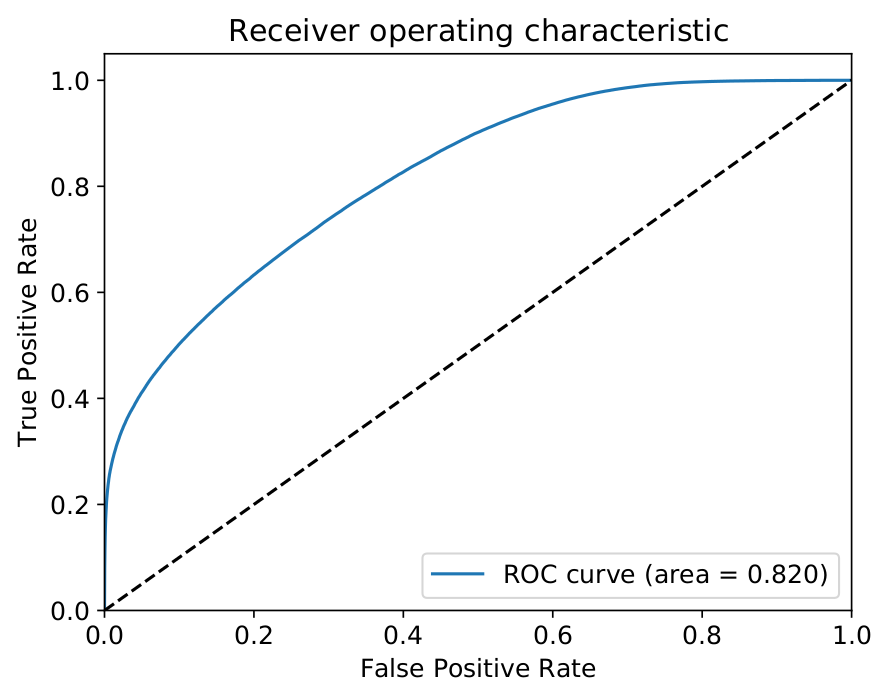
\includegraphics[width=8cm]{assets/chap03/roc.png}
    \caption{Example of a ROC curve.}
    \label{fig:ch_3_roc}
\end{figure}
The AUC score of a ROC curve can be used to determine overfitting, e.g., when the AUC score of the training data set is higher than that of the validation data set.

The confusion matrix is a table layout, where each row of the matrix represents the instance counts in a predicted class, while each column represents the counts in an actual class.

Assume a classifier has been trained to distinguish between cats, dogs and rabbits with a sample of 27 animals, where 8 are cats, 6 dogs and 13 rabbits.

\begin{table}[h]
    \caption[Confusion matrix]{Confusion matrix with prediction results of the classifier that distinguishes between cats, dogs and rabbits. Source: \cite{wiki:confusionmatrix}}
    \label{tab:ch_3_confusion_matrix}
    \begin{center}
        \begin{tabular}{|c|c|c|c|c|}
            \hhline{~~---}
            \multicolumn{2}{c|}{}&\multicolumn{3}{c|}{\textbf{Actual class}}\\
            \hhline{~~---}
            \multicolumn{2}{c|}{}&\textbf{Cat}&\textbf{Dog}&\textbf{Rabbit}\\
            \hline
            \multirow{3}{*}{\rotatebox[origin=c]{90}{\textbf{\shortstack{Predicted\\class}}}} & \textbf{Cat} & \textbf{5} & 2 & 0\\
            \hhline{~----}
             & \textbf{Dog} &3&\textbf{3}&2\\
            \hhline{~----}
             & \textbf{Rabbit} &0&1&\textbf{11}\\
            \hline
        \end{tabular}
    \end{center}
\end{table}

Reading the columns of Table \ref{tab:ch_3_confusion_matrix} vertically, the classifier predicted that of the 8 actual cats 3 were dogs, of the actual 6 dogs 2 were cats and 1 rabbit and of the actual 13 rabbits 2 were dogs. The correct predictions are highlighted in bold in the diagonal of the table, the incorrect predictions are represented by values outside the diagonal.